\section{Attacks}

%%%%%%%%%%%%%%%%%%%%%%%%%%%%%%%%%%%%%%%%%%%%%%%%%%%%%%%%%%%%%%%%%%%%%%%%%%%%%%
\subsection{Attack trees}

\begin{frame}
\includeimage[width=\linewidth,height=0.8\textheight]{attack-tree-admin}
\note{
\begin{block}{What is it?}
Model describing how an \emph{asset} can be attacked.
\end{block}
\begin{block}{Goal}
Used to determine and understand threats that may arise.
\end{block}
}
\end{frame}

%%%%%%%%%%%%%%%%%%%%%%%%%%%%%%%%%%%%%%%%%%%%%%%%%%%%%%%%%%%%%%%%%%%%%%%%%%%%%%
\subsection{Threat agents}

\begin{frame}
\frametitle{Threat agents}
\begin{columns}
\begin{column}{0.6\linewidth}
\includeimage[width=\linewidth,height=4cm]{hacker}
\end{column}
\begin{column}{0.4\linewidth}
\includeimage[width=\linewidth,height=3cm]{yes-i-can}
\end{column}
\end{columns}
\note{
\begin{description}
\item[External threats]
	\hfill
	\begin{itemize}
	\item internet users
		\begin{itemize}
		\item white-hat
		\item black-hat
		\end{itemize}
	\item viruses
	\end{itemize}
\item[Internal threats]
	Unsatisfied employees (intranet users)
\item[Reason]
	To show off, break things
\end{description}
}
\end{frame}

\begin{frame}
\frametitle{Threat agents}
\begin{columns}
\begin{column}{0.6\linewidth}
\includeimage[width=\linewidth,height=4cm]{organized-crime}
\includeimage[width=\linewidth,height=4cm]{competitors}
\end{column}
\begin{column}{0.4\linewidth}
\includeimage[width=0.6\linewidth]{money}
\end{column}
\end{columns}
\note{
\begin{description}
\item[External threats]
	\hfill
	\begin{itemize}
	\item organized crime
	\item competitor
	\end{itemize}
\item[Reason]
	Gain
	\begin{itemize}
	\item financial
	\item information
	\item competition
	\end{itemize}
\end{description}
\begin{block}{Impact}
Threat agents have different skills, resources and different motivations that
may influence risk.
\end{block}
}
\end{frame}

\begin{frame}
\frametitle{Threat agents}
\begin{columns}
\begin{column}{0.4\linewidth}
\includeimage[width=\linewidth,height=4cm]{no-electricity}
\end{column}
\begin{column}{0.6\linewidth}
%\includeimage[width=\linewidth,height=4cm]{crew}
\includeimage[width=\linewidth,height=3.5cm]{mean-old-lady}
\end{column}
\end{columns}
\note{
\begin{description}
\item[Internal threats]
	Employees, crew
\item[Technical failure]
	\hfill
	\begin{itemize}
	\item loss of essential services (electricity, etc.)
	\item hardware failure
	\item software failure
	\end{itemize}
\item[Reason]
	Unintentional, accident
\end{description}
}
\end{frame}

\begin{frame}
\frametitle{Threat agents}
\includeimage[height=0.3\textheight]{disaster}
\pause
\fontsize{14pt}{7.2}\selectfont
\begin{exampleblock}{In {\bfseries Belgium} between 1980-2010}
\begin{center}
\begin{tabular}{lr}
No of events: & 39 \\
Economic damage per year: & 69 million \\
Gross National Product: & $\sim$ 400 milliards \\
% vs Gross National Product (0.00017)
\end{tabular}
% Source:
% http://www.preventionweb.net/english/countries/statistics/?cid=17
\end{center}
\end{exampleblock}
\note{
\begin{description}
\item[Natural threats]
	(disasters)
	\newline Storms, floods, earthquakes, ...
	\newline Insignificant: 0.00017 of GNP
\end{description}
}
\end{frame}

%%%%%%%%%%%%%%%%%%%%%%%%%%%%%%%%%%%%%%%%%%%%%%%%%%%%%%%%%%%%%%%%%%%%%%%%%%%%%%
\subsection{Risk}

\begin{frame}
\frametitle{What is a \emph{risk}?}
\begin{quote}
The probable {\Large frequency} and probable {\Large magnitude} of {\Large
future loss}.
\textit{-- The Open Group}
\end{quote}
% Source:
% http://www.riskmanagementinsight.com/media/docs/FAIR_introduction.pdf
\note{
Just a good definition.
Explanation in the next slide.
}
\end{frame}

\begin{frame}
\begin{Large}
\[ \text{risk} = \text{likelihood} * \text{impact} \]
\end{Large}
\note{
\begin{itemize}
\item Likelihood: probability of a successful attack
	\\ Influenced by threat agent skills and vulnerability factors
\item Impact: how much damage the attack causes
\end{itemize}
\begin{columns}
\begin{column}{0.5\linewidth}
\par\textbf{Vulnerability factors}
\begin{itemize}
\item Ease of discovery
\item Ease of exploit
\item Awareness
\item Intrusion detection
\end{itemize}
\end{column}
\begin{column}{0.5\linewidth}
\par\textbf{Impact factors}
\begin{itemize}
\item Loss of confidentiality, integrity, availability, accountability
\item Financial damage
\item Reputation damage
\item Privacy violation
\end{itemize}
\end{column}
\end{columns}
}
\end{frame}

%%%%%%%%%%%%%%%%%%%%%%%%%%%%%%%%%%%%%%%%%%%%%%%%%%%%%%%%%%%%%%%%%%%%%%%%%%%%%%
\subsection{Context of web applications}

\subsubsection{Network}
\begin{frame}
\includeimage[width=\linewidth,height=0.75\textheight]{client-server}
\note{
\begin{itemize}
\item Applications available on the internet
\item Anyone can access the application
\end{itemize}
}
\end{frame}

\subsubsection{Architecture of a web application}

\begin{frame}
\includeimage[width=\linewidth,height=0.8\textheight]{archi-webapplication}
\note{
\begin{itemize}
\item Browser: the client, uses scripting
\item Router: connected to the browser (by WiFi) - LAN
\item Internet: not detailed here - WAN
\item DMZ: demilitarized zone {\small (exposed subnetwork)}
\item Web Application Firewall, IDS, Load Balancer
\item Application Server: with the contained application
\end{itemize}
\begin{block}{Points of failure}
Any component may fail; will the web site continue to work?
\par It is possible to intervene at multiple levels.
\begin{description}
\item[Single point of failure]
A part of a system that prevents the entire system from working when it fails.
Solution: duplication.
\end{description}
\end{block}
}
\end{frame}

%%%%%%%%%%%%%%%%%%%%%%%%%%%%%%%%%%%%%%%%%%%%%%%%%%%%%%%%%%%%%%%%%%%%%%%%%%%%%%
\subsection{OWASP - Top 10}

\begin{frame}
\centering
{\bfseries\usebeamercolor[fg]{block title}O}pen
{\bfseries\usebeamercolor[fg]{block title}W}eb
{\bfseries\usebeamercolor[fg]{block title}A}pplication
{\bfseries\usebeamercolor[fg]{block title}S}ecurity
{\bfseries\usebeamercolor[fg]{block title}P}roject
\includeimage[width=0.5\linewidth,height=3cm]{logo-owasp}
\begin{center}
\url{https://www.owasp.org/}
\end{center}
\note{
\begin{block}{OWASP}
\begin{itemize}
\item Standards
\item Libraries
\item Books
\item Etc.
\end{itemize}
\end{block}
\begin{block}{Project: Top 10}
OWASP compiles a top 10 of most critical web application \emph{risks}.
\end{block}
}
\end{frame}

\begin{frame}
\frametitle{Top 10}
\begin{enumerate}
\item Injection
\item Cross-site Scripting (XSS)
\item Authentication and Session Management
\item Insecure Direct Object References
\item Cross-site Request Forgery (CSRF)
\item Security Misconfiguration
\item Insecure Cryptographic Storage
\item Failure to Restrict URL Access
\item Insufficient Transport Layer Protection
\item Unvalidated Forwards and Redirects
\end{enumerate}
\note{
\begin{block}{Project: Top 10}
Top 10 of most critical web application \emph{risks}.
\end{block}
\begin{block}{Demo application}
\begin{itemize}
\item Built with security flaws for the demo
\item Hotel rating web site
\item Shown hotels must be approved by an administrator
\end{itemize}
\end{block}
}
\end{frame}

\begin{frame}
\frametitle{Demo website}
\begin{description}
\item[Theme]
	Hotel rating website
	\hfill
	\begin{itemize}
	\item Any user can post comments
	\item Administration to approve new hotels
	\item Unapproved hotels are not listed
	\end{itemize}
\item[Technologies]
	Java website
	\hfill
	\begin{itemize}
	\item Spring - core, MVC
	\item Hibernate - h2database
	\item JSP
	\end{itemize}
\end{description}
\note{
Used technologies, etc. for the demo.
}
\end{frame}

\begin{frame}
\includeimage[width=\linewidth,height=0.75\textheight]{demo-website}
\note{
Screenshot of the demo website.
}
\end{frame}

\subsubsection{Attack 1 - Injection}

\begin{frame}
\frametitle{1. Injection}
\includeimage[scale=0.5]{client-server-injection}
\note{
\textbf{Injection} consists in sending untrusted data to an interpreter.
Attacker enters code to execute into input fields.
\begin{example}
Send code directly to some interpreter.
\end{example}
\begin{block}{Impacts}
Data loss, corruption, lack of accountability, etc.
\end{block}
\begin{alertblock}{Risks}
Easy to exploit, has a severe impact, it is quite common.
\end{alertblock}
}
\end{frame}

\defverbatim[colored]\Lst{
\begin{lstlisting}[style=beamer]
String query = "select * from users"
	+ " where user_name = '" @+ name +@ "'"
	+ " and password = '" @+ password +@ "'";
\end{lstlisting}
}
\begin{frame}
\begin{exampleblock}{\emph{THE} password}
\includeimage[height=0.4\textheight]{the-password}
\pause
\begin{embeddedcode}{bad}
\Lst
\end{embeddedcode}
\end{exampleblock}
\note{
%\begin{exampleblock}{SQL injection - demo}
%Getting the users' passwords as administrator.
%\end{exampleblock}
\begin{exampleblock}{JPQL injection - demo}
Searching hotels that have a manager that has the same password as a given
user.
\end{exampleblock}
The \emph{concatenation} is the cause of the injection: the query
is built from unvalidated input.
}
\end{frame}

\defverbatim[colored]\Lst{
\begin{lstlisting}[style=beamer]
String query = "select * from users"
	+ " where @user_name = ?@"
	+ " and @password = ?@";
PreparedStatement st = con.prepareStatement(query);
@st.setString(1, name);@
@st.setString(2, password);@
ResultSet rs = st.executeQuery();
\end{lstlisting}
}
\begin{frame}
\begin{embeddedcode}{good}
\Lst
\end{embeddedcode}
\vspace{1cm}
\pause
\begin{itemize}
\item Parametrized interface
\item Escaping routines
\item White list validation
\end{itemize}
\note{
\begin{block}{Using parametrized interface}
Usage of placeholders for values let's the interpreter escape and validate
input values.
\end{block}
\begin{block}{Escaping routines}
Some languages have special functions to escape manually values.
\end{block}
\begin{block}{White list validation}
List of valid input patterns.
\end{block}
}
\end{frame}

\subsubsection{Attack 2 - XSS}

\begin{frame}
\frametitle{2. XSS}
\includeimage[scale=0.5]{client-server-xss}
\note{
\textbf{Cross-site scripting} allows attackers to inject code into the page
sent to the user. The injected code can be a script interpreted by the
browser.
\begin{example}
The attacker sends a script to a web page. Users who download the code execute
it in their browser.
\end{example}
\begin{block}{Impacts}
Hijack user sessions, change content, redirect the user.
\end{block}
\begin{alertblock}{Risks}
The most widespread vulnerability.
It requires an average knowledge to be exploited and the impacts are moderate.
\end{alertblock}
}
\end{frame}

\defverbatim[colored]\LstBad{
\begin{lstlisting}[style=beamer]
<div>
	@${hotel.description}@
</div>
\end{lstlisting}
}
\defverbatim[colored]\LstGood{
\begin{lstlisting}[style=beamer]
<div>
	@<c:out value="${hotel.description}" />@
</div>
\end{lstlisting}
}
\begin{frame}
\begin{embeddedcode}{bad}
\LstBad
\end{embeddedcode}
\badgoodsep
\begin{embeddedcode}{good}
\LstGood
\end{embeddedcode}
\note{
{\bfseries JSP page}\par
Unescaped included text in a JSP.
\begin{exampleblock}{Getting the user's cookies - demo}
Just use \lstinline!document.cookie! in JavaScript and send it to
\emph{another server}.
\end{exampleblock}
\begin{block}{Escaping the values}
All the values should be escaped before sending them to the users.
\end{block}
\begin{block}{White list validation}
Output values can be white listed, but this is not a complete defence against
XSS as sometimes special characters must be accepted.
\end{block}
}
\end{frame}

\subsubsection{Attack 3 - Authentication and Session Management}

\begin{frame}
\frametitle{3. Authentication and Session Management}
\includeimage[scale=0.5]{client-server-session}
\note{
The attacker uses flaws in the \textbf{authentication or session management}
implemented for a given web site to steal someone else's identity.
\begin{example}
\begin{itemize}
\item Session hijacking
\item Session fixation
\end{itemize}
\end{example}
\begin{block}{Impacts}
Once an account has been stolen, the attacker may do \emph{anything} the user
can do.
\end{block}
\begin{alertblock}{Risks}
The impact is severe, this attack is common.
\end{alertblock}
}
\end{frame}

\defverbatim[colored]\Lst{
\begin{lstlisting}[style=beamer]
http://host.com/page@;jsessionid=dfd4fa35df@...
\end{lstlisting}
}
\begin{frame}
\begin{columns}
\begin{column}{0.3\linewidth}
\centering\huge\bfseries
XSS
\end{column}
\begin{column}{0.6\linewidth}
\includeimage[width=\linewidth,height=2cm]{cybercafe}
\end{column}
\end{columns}
\vspace{3mm}
\Lst
\badgoodsep
\begin{center}
\huge\bfseries
Good authentication mechanism
\end{center}
\note{
\begin{exampleblock}{Public computer}
Forgetting to log out...
\end{exampleblock}
\begin{exampleblock}{Session fixation}
In older application server, the session ID could be set using the URL.
You could send that URL to someone else.
\end{exampleblock}
\pause
\begin{exampleblock}{XSS session hijacking - demo}
The user's session can be obtained using XSS.
\end{exampleblock}
\hrule
\begin{block}{Good authentication mechanism}
\begin{itemize}
\item Use a proven authentication mechanism
\item Prevent \emph{XSS attacks}
\item Good session timeouts and accessible log out buttons
\end{itemize}
\end{block}
}
\end{frame}

\subsubsection{Attack 4 - Insecure Direct Object References}

\defverbatim[colored]\Lst{
\begin{lstlisting}[style=beamer]
http://myhotel.com/user/@152@
\end{lstlisting}
}
\begin{frame}
\frametitle{4. Insecure Direct Object References}
\begin{columns}
\begin{column}{0.3\linewidth}\end{column}
\begin{column}{0.5\linewidth}
\Lst
\end{column}
\end{columns}
\note{
The attacker changes a parameter in the request to obtain a \textbf{direct
object reference} that they should not be able to access.
\begin{example}
Replace some object identifier in the request.
\end{example}
\begin{block}{Impacts}
Compromise the data that can be referenced.
\end{block}
\begin{alertblock}{Risks}
Easy to exploit and detect. The impact is moderate.
\end{alertblock}
}
\end{frame}

\begin{frame}
\begin{center}
{\Huge\bfseries Check permissions}
\end{center}
\note{
\begin{block}{Missing access verification}
Often objects are retrieved by their ID, the developer can forget to check
whether the user is allowed to see that object.
\end{block}
\hrule
\begin{exampleblock}{An unvalidated hotel - demo}
See an unvalidated hotel as a normal user.
\end{exampleblock}
\hrule
\begin{block}{\textbf{Check permissions}}
Check whether the user has the permissions to access the object before
manipulating it.
\end{block}
\begin{block}{References by session}
Use indirect references for each session.
\end{block}
}
\end{frame}

\subsubsection{Attack 5 - CSRF}

\begin{frame}
\frametitle{5. CSRF}
\includeimage[scale=0.5]{client-server-csrf}
\note{
\textbf{Cross-site Request Forgery} consists in generating requests when the
user visits the attacker's web page.
\begin{example}
\begin{itemize}
\item A user visits the attacker's web page
\item The requested page contains tricks to submit requests to the attacked
web site as the visiting user
\end{itemize}
\end{example}
\begin{block}{Impacts}
The attacker may perform actions as the victim.
\end{block}
\begin{alertblock}{Risks}
Widespread and easy to detect, the impact is moderate.
\end{alertblock}
}
\end{frame}

\defverbatim[colored]\LstBad{
\begin{lstlisting}[style=beamer]
<img src="http://@host.com@/forum/thread1/
@addComment@?text=hello%20world" alt="" />
\end{lstlisting}
}
\defverbatim[colored]\LstGood{
\begin{lstlisting}[style=beamer]
<form @method="post"@ action="addComment">
	<input @type="hidden"@ name="token" @value="<random>"@ />
	...
</form>
\end{lstlisting}
}
\begin{frame}
\begin{embeddedcode}{bad}
\LstBad
\end{embeddedcode}
\badgoodsep
\begin{embeddedcode}{good}
\LstGood
\end{embeddedcode}
\note{
\begin{exampleblock}{Post a comment}
The attacker's page may contain:
\end{exampleblock}
\hrule
\begin{block}{Unpredictable token}
Each request contains a field that is a token linked to the session of
the user, the attacker's website will not be able to generate the correct
requests.
\newline
Tokens can be unique by session or by request.
\par
The token is usually stored in a cookie (preferably HTTP-only).
In forms, a hidden field contains the same value.
When the request is sent, both values are compared.
\par
Only the session ID is stored in the cookie; the session information is
stored only on the application server.
\end{block}
}
\end{frame}

\subsubsection{Attack 6 - Security Misconfiguration}

\begin{frame}
\frametitle{6. Security Misconfiguration}
\includeimage[width=0.7\linewidth]{misconfiguration}
\note{
\textbf{Security configuration} can happen at any level: the application, the
web server, the framework, etc.
The default behavior is not always the wanted one.
\begin{example}
\begin{itemize}
\item Accessing: default accounts, unprotected files and directories
\item Gaining information: versions, stack traces, debug messages
\end{itemize}
\end{example}
\begin{block}{Impacts}
Attackers can gain unauthorized access, the system can be compromised.
\end{block}
\begin{alertblock}{Risks}
Easy to exploit and to detect.
\end{alertblock}
}
\end{frame}

\begin{frame}
\includeimage[height=0.7\textheight,width=\linewidth]{out-of-the-box}
\note{
The out-of-the-box configuration is not always the best.
}
\end{frame}

\begin{frame}
\includeimage[width=\linewidth,height=0.7\textheight]{webpage-stacktrace}
\pause
\raggedleft\Large
... more information for the attacker
\note{
\begin{block}{Outdated libraries}
Bugs are published for known libraries and applications.
\end{block}
\begin{exampleblock}{Stack trace}
A stack trace may contain the used parameters, references to libraries, etc.
\end{exampleblock}
\hrule
\begin{block}{Up-to-date system}
Keep the used software up to date and manage versions.
\end{block}
\begin{block}{Good architecture}
Good separation between components is more secure.
\end{block}
\begin{block}{Automated scan}
Automated scans can detect misconfigurations and missing patches.
\end{block}
}
\end{frame}

\subsubsection{Attack 7 - Insecure Cryptographic Storage}

\begin{frame}
\frametitle{7. Insecure Cryptographic Storage}
\begin{center}
\begin{tabular}{|l|l|l|c|}
\hline
ID & NAME & PASSWORD & \ldots \\
\hline
1 & admin & 2ezf5zf2d & \ldots \\
2 & jacky & toto & \ldots \\
3 & k & 123456 & \ldots \\
\hline
\end{tabular}
\end{center}
\note{
Sensitive data is stored \textbf{insecurely without crypting}.
\begin{example}
All data is readable by the attacker once he gains access to it.
\end{example}
\begin{block}{Impacts}
Stolen data is compromised.
\end{block}
\begin{alertblock}{Risks}
All unencrypted data is compromised.
The attack is however difficult to perform.
\end{alertblock}
}
\end{frame}

\begin{frame}
\includeimage[height=0.7\textheight,width=0.9\linewidth]{rainbow-table-example}
\note{
\begin{exampleblock}{Unencrypted passwords}
After dumping the table \texttt{USERS}, the passwords might be stored in
plain text.
\end{exampleblock}
\begin{exampleblock}{\textbf{Rainbow tables}}
Precomputed table for decoding hashed values.
\href{http://www.md5this.com/list.php?page=133&key=1}{\texttt{md5this.com}}
\end{exampleblock}
}
\end{frame}

\begin{frame}
\includeimage[height=0.6\textheight,width=0.8\linewidth]{backup}
\note{
\begin{exampleblock}{Unencrypted backup}
The database backup is lost.
\end{exampleblock}
}
\end{frame}

\begin{frame}
\frametitle{Hash + Salt}
\begin{center}
hash("hello") = "b1946ac92492d2347c6235b4d2611184" \\[1cm]
\begin{flushright}
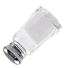
\includegraphics[width=1.5cm]{img/icon-salt}
\end{flushright}
hash("hello", salt1) = "5b1cdd3502528d92b16925aebb99e785" \\
hash("hello", salt2) = "72a11579b4256c9f604875ea17dbd803" \\
\end{center}
\note{
Ensure passwords are hashed with a standard algorithm and a different salt is
used for each password.
\begin{itemize}
\item Prevents \emph{rainbow table} attacks
\item Both the hash and salt are stored in a database
\end{itemize}
}
\end{frame}

\subsubsection{Attack 8 - Failure to Restrict URL Access}

\defverbatim[colored]\Lst{
\begin{lstlisting}[style=beamer]
http://myhotel.com/@admin@
\end{lstlisting}
}
\begin{frame}
\frametitle{8. Failure to Restrict URL Access}
\begin{columns}
\begin{column}{0.3\linewidth}\end{column}
\begin{column}{0.5\linewidth}
\Lst
\end{column}
\end{columns}
\note{
\textbf{URL access is not restricted} to functions requiring permissions.
\begin{example}
The attacker changes his URL to a privileged page.
\end{example}
\begin{block}{Impacts}
Administrative functions may become available to the attacker.
\end{block}
\begin{alertblock}{Risks}
Easy to exploit, but the flaw is uncommon.
\end{alertblock}
}
\end{frame}

\begin{frame}
\begin{center}
{\Huge\bfseries Authorization}
\end{center}
\note{
\begin{exampleblock}{Administration page}
\url{http://myhotel.com/admin} is not referenced from any other page, but
the authentication is not enforced.
\end{exampleblock}
\hrule
\begin{block}{Check permissions}
Authorization mechanisms should be used.
\end{block}
}
\end{frame}

\subsubsection{Attack 9 - Insufficient Transport Layer Protection}

\begin{frame}
\frametitle{9. Insufficient Transport Layer Protection}
\includeimage[width=0.8\linewidth]{wifi-sniffing}
\note{
\textbf{Traffic is unprotected} and anyone sniffing the network can see the
data in transit.
\begin{example}
\begin{itemize}
\item Sniffing the WiFi network
\item Scanning for HTTP requests
\item Analyzing conversations
\end{itemize}
\end{example}
\begin{block}{Impacts}
Account theft, expose individual user's data.
\end{block}
\begin{alertblock}{Risks}
Detectable using any sniffer.
However, often difficult to exploit.
\end{alertblock}
}
\end{frame}

\begin{frame}
\includeimage[width=0.5\linewidth]{https}
\note{
The attacker can see the data that is sent over the network.
\begin{exampleblock}{Sniffing passwords}
Sniff the network and find HTTP requests containing "password".
\end{exampleblock}
\hrule
\begin{block}{HTTP\textbf{S}}
SSL/TLS can be used to secure the connection.
\begin{itemize}
\item \emph{secure} cookies will not be sent through an unencrypted connection
\item Ensure that certificates are valid
\end{itemize}
\end{block}
}
\end{frame}

\subsubsection{Attack 10 - Unvalidated Forwards and Redirects}

\defverbatim[colored]\Lst{
\begin{lstlisting}[style=beamer]
http://host.com/forward.jsp?@fwd=admin.jsp@
\end{lstlisting}
}
\begin{frame}
\frametitle{10. Unvalidated \textbf{Forwards} and Redirects}
\includeimage[scale=0.5]{webapp-forward}
\vspace{6mm}
\Lst
\note{
A URL may appear as trustworthy, but it contains an \textbf{unvalidated
forward or redirect}.
\begin{example}
The attacker may bypass authorization for \texttt{admin.jsp}.
\end{example}
\begin{block}{Impacts}
Tricking victims into disclosing information, unsafe forwards may allow access
control bypass.
\end{block}
\begin{alertblock}{Risks}
Easy to detect, uncommonly present.
\end{alertblock}
}
\end{frame}

\defverbatim[colored]\Lst{
\begin{lstlisting}[style=beamer]
https://@bank.com/secured@/../redirect
?@url=http://evil-bank.com/secured@
\end{lstlisting}
}
\begin{frame}
\frametitle{10. Unvalidated Forwards and \textbf{Redirects}}
\includeimage[scale=0.45]{webapp-redirect}
\vspace{4mm}
\Lst
\note{
\begin{example}
Placing a URL with a redirect that seems trustworthy redirecting to a
malicious page.
\end{example}
\begin{exampleblock}{Malicious site}
Redirect to a malicious website using:
\\ \url{http://bank.com/redirect?url=evil-bank.com}
\end{exampleblock}
\hrule
\begin{block}{Avoid redirects and forwards}
Avoid \emph{parametrized} redirects and forwards.
\end{block}
\begin{block}{Authorization}
Validate and authorize the user after each redirect.
\end{block}
\begin{exampleblock}{Map input values}
Map input values to the actual URLs.
\end{exampleblock}
}
\end{frame}

%%%%%%%%%%%%%%%%%%%%%%%%%%%%%%%%%%%%%%%%%%%%%%%%%%%%%%%%%%%%%%%%%%%%%%%%%%%%%%
\subsection{DoS}

\begin{frame}
\begin{center}
\Huge\bfseries
What about just crashing the system?
\end{center}
\note{
Transition...
}
\end{frame}

\begin{frame}
\frametitle{Denial of Service (DoS)}
\includeimage[width=0.8\linewidth,height=0.8\textheight]{overwhelmed-donkey}
\note{
Attack that aims to bring down (or make unavailable) some service usually by
causing server overload.
\begin{quote}
An \emph{important load} causes \emph{service overload}.
\end{quote}
\begin{itemize}
\item SYN flood
\item Application level flood
\item R-U-Dead-Yet
	\newline
	(never-ending POST transmissions,
	example: \href{http://ha.ckers.org/slowloris/}{Slowloris})
\item DDoS
\item Unintentional DoS
\end{itemize}
}
\end{frame}

\begin{frame}
\begin{columns}
\begin{column}{0.5\linewidth}
\includeimage[width=\linewidth,height=0.5\textheight]{anonymous-group}
\end{column}
\pause
\begin{column}{0.5\linewidth}
\includeimage[width=\linewidth]{dos-unintentional}
\end{column}
\end{columns}
\note{
\frametitle{Denial of Service - example}
\begin{exampleblock}{DDoS}
The anonymous group attack.
\end{exampleblock}
\begin{exampleblock}{Unintentional DoS}
\begin{itemize}
\item page linked from \url{http://slashdot.org}
\item \href{http://www.joueurdugrenier.fr/}{Joueur du Grenier} - new video
\end{itemize}
\end{exampleblock}
\hrule
\begin{block}{Denial of Service - prevention}
\begin{itemize}
\item Firewall
\item Intrusion Prevention System
\item Black-holing
\end{itemize}
\end{block}
}
\end{frame}

%%%%%%%%%%%%%%%%%%%%%%%%%%%%%%%%%%%%%%%%%%%%%%%%%%%%%%%%%%%%%%%%%%%%%%%%%%%%%%
\subsection{MitM}

\begin{frame}
\begin{center}
\Huge\bfseries
And modifying the content?
\end{center}
\note{
Transition...
}
\end{frame}

\begin{frame}
\frametitle{Man in the Middle attack}
\includeimage[height=0.6\textheight]{phone-tapping}
\note{
The attacker plays the role of the server to the client and the role of the
client to the server.
All communication transits through the attacker who can modify messages as
they are sent.
\begin{exampleblock}{Public WiFi}
Vulnerable on public WiFi networks.
\\ Tools such as \texttt{ettercap} allow to perform the attack.
\end{exampleblock}
\begin{exampleblock}{Common example}
Submitting a bank transfer request and modifying the parameters.
\end{exampleblock}
\hrule
\begin{block}{Prevention}
Use cryptography: HTTPS, PKI (Public Key Infrastructure)
\end{block}
}
\end{frame}

%%%%%%%%%%%%%%%%%%%%%%%%%%%%%%%%%%%%%%%%%%%%%%%%%%%%%%%%%%%%%%%%%%%%%%%%%%%%%%
\subsection{Social engineering}

\begin{frame}
\frametitle{Social engineering}
%\includeimage[width=0.8\linewidth]{social-engineering}
\includeimage[width=0.8\linewidth]{networking-sites}
\note{
\textbf{Social engineering} consists in manipulating people so they divulge
confidential information.
\\ Similar to fraud.
}
\end{frame}

\begin{frame}
\includeimage[height=0.75\textheight,width=\linewidth]{xkcd538_security}
\note{
Recall how you can break strong encryption.
\begin{block}{E-mail}
Once the e-mail account has been hacked, you can reset the password for other
services that would send an e-mail when recovering a lost password.
\par
A secret question could be targeted by social engineering.
\end{block}
}
\end{frame}

%TODO : Garder cette frame ? ajouter un titre
% si vous la jettez, gardez les notes!
\begin{frame}
\includeimage[width=0.8\linewidth,height=0.6\textheight]{hannibal-lecter}
\begin{quote}
\begin{center}
Quid pro quo, Clarice...
\end{center}
\end{quote}
\note{
\begin{description}
\item[Pretexting]
Using an invented scenario (the pretext) to engage a targeted victim in
a manner that increases the chance the victim will divulge information
or perform actions that would be unlikely in ordinary circumstances.
\item[Phishing]
See the next point.
\item[Quid pro quo]
Something for something:
Help a user solve a problem, they might give you passwords in exchange.
\end{description}
\begin{block}{Protection}
\begin{itemize}
\item Rising awareness {\small (sensibilization)}
\item Framework of trust
\end{itemize}
\end{block}
}
\end{frame}

%%%%%%%%%%%%%%%%%%%%%%%%%%%%%%%%%%%%%%%%%%%%%%%%%%%%%%%%%%%%%%%%%%%%%%%%%%%%%%
\subsubsection{Phishing}

\begin{frame}
\frametitle{Phishing}
\includeimage[height=0.75\textheight,width=\linewidth]{phishing-mail}
\note{
\textbf{Phishing} is the attempt to acquire user information through
masquerading as a legitimate web site.
\begin{itemize}
\item Cloned websites
\item Link manipulation
\item Phone phishing
\item Etc.
\end{itemize}
\hrule
\begin{block}{Phishing - prevention}
\begin{itemize}
\item Education
\item Help to identify legitimate web sites
\end{itemize}
\end{block}
}
\end{frame}

\begin{frame}
\includeimage[height=0.75\textheight,width=\linewidth]{cloned-website}
\note{
A \emph{cloned} website.
}
\end{frame}

%%%%%%%%%%%%%%%%%%%%%%%%%%%%%%%%%%%%%%%%%%%%%%%%%%%%%%%%%%%%%%%%%%%%%%%%%%%%%%
\subsection{Other attacks}

\begin{frame}
\frametitle{Brute force}
%\includeimage[height=0.7\textheight]{letstryallthepasswords}
\includeimage[height=0.7\textheight]{hulk-smash}
\note{
\begin{block}{Try all the passwords}
Try all the possible combinations.
\newline
$k^n$ where $k$ is the size of the alphabet and $n$ the length of the
password.
\end{block}
\begin{block}{Dictionary attack}
Try a list of common passwords.
\\ English language contains only hundreds of thousands words.
\end{block}
}
\end{frame}

\defverbatim[colored]\Lst{
\begin{lstlisting}[style=beamer]
http://host.com/forum/download.jsp
?@path=/etc/shadow@
\end{lstlisting}
}
%TODO : Agrandir le code
% jeter cette faille?
\begin{frame}
\frametitle{Path traversal}
\Lst
\note{
An input is a relative unvalidated path.
You can download or upload any file that the server contains.
\begin{exampleblock}{Download form}
Get a file uploaded to a forum... or the password file.
\end{exampleblock}
}
\includeimage[scale=0.3]{etc-shadow}

\end{frame}

%TODO : Exemple rest api ? Change title ?
% jeter cette faille?
\begin{frame}
\frametitle{Failure to restrict automation}
\begin{itemize}
\item Spamming
\item REST API
\end{itemize}
\pause
\vspace{2cm}
\includeimage[width=0.6\linewidth]{recaptcha-example}
\note{
The web site is not protected against automation.
\begin{itemize}
\item Common for REST API
\item Programs may overload the website unintentionally
	\newline
	(Fix: maximum number of requests per IP for a time period)
\end{itemize}
\begin{exampleblock}{Captcha - prevention}
Challenge-response test easy for humans, difficult for machines.
\end{exampleblock}
\begin{block}{Captcha - cracking}
The attacker has to make a website with high traffic on it (image boards,...). Once done, the evil website can present a captcha from another website. The users visiting the evil website answer the captcha and the evil website can use this answer to crack the protection of the attacked website.
\end{block}
}
\end{frame}

\begin{frame}
\frametitle{And so on...}
\includeimage[width=0.9\linewidth,height=0.85\textheight]{attack-tag-cloud}
\note{
As technology evolves, new forms of attacks appear.
\par
Instead of trying to fix vulnerabilities, focus on establishing strong
security controls.
}
\end{frame}

%%%%%%%%%%%%%%%%%%%%%%%%%%%%%%%%%%%%%%%%%%%%%%%%%%%%%%%%%%%%%%%%%%%%%%%%%%%%%%
\subsection{Common points}

\begin{frame}
\frametitle{Common points}
\begin{itemize}
\item<+-> Improper input validation
\item<+-> Missing authorization checks
\item<+-> Misconfiguration
\item<+-> Other assumptions
\item<+-> Education factor {\small (social engineering)}
\end{itemize}
\note{
Bullet points.
}
\end{frame}

